\section{Theoretical Framework}
\label{sec:theory}

This section establishes the mathematical foundations required for the decision model applied in section \ref{sec:decision_model}. The decision space is formally defined, along with the Ordered Weighted Averaging (OWA) operator and its variant, the Weighted OWA (WOWA). Finally, for a fixed finite choice set, an exact geometric transformation is derived that represents WOWA as an equivalent higher-dimensional OWA with a unified weight vector, thereby enabling the Linear Programming analysis from section \ref{sec:selection}.

\subsection{Decision Space and Notation}
%!SYNTHESIZING judgments is an important part of multiple criteria decision-making methods. The typical situation concerns individuals that form quantifiable judgments about a measure of an object (weight, length, area, height, volume, importance, or other attributes, for instance, in the framework of a hierarchy)

Let $A = \{a_1, a_2, \dots, a_N\}$ be a finite set of $N$ alternatives and $C = \{c_1, c_2, \dots, c_M\}$ be a set of $M$ criteria. The evaluation of alternatives is represented by a decision matrix $\mathbf{X}=(x_{ij})\in [0,1]^{N \times M}$, where $x_{ij}$ denotes the normalized performance of alternative $a_i$ with respect to criterion $c_j$. It is assumed, without loss of generality, that all criteria are of the ``benefit'' type (higher values are strictly preferred).

\[\mathbf{X}=
	\setlength{\arraycolsep}{5pt} % adjust spacing if desired
	\begin{array}{c@{\,}l}
		% Left block: matrix with column labels underneath
		\begin{array}{c}
			\begin{pmatrix}
					x_{11} & x_{12} & \cdots & x_{1M} \\
					x_{21} & x_{22} & \cdots & x_{2M} \\
					\vdots & \vdots & \ddots & \vdots \\
					x_{N1} & x_{N2} & \cdots & x_{NM}
			\end{pmatrix} \\[2mm] % vertical space between matrix and column labels
			\begin{array}{llll}
					\scriptstyle c_1 \hspace{1mm} & \hspace{1mm}\scriptstyle c_2 \hspace{1mm} & \hspace{1mm}\cdots & \hspace{1mm}\scriptstyle c_M
			\end{array}
		\end{array}
		% Right block: row labels aligned with matrix rows
		\hspace{-2.5mm}
		\begin{array}{l}
			\scriptstyle a_1    \\%[-2.5mm]
			\scriptstyle a_2    \\%[-2.5mm]
			\scriptstyle \vdots \\%[-2.5mm]
			\scriptstyle a_N    \\
			\\
		\end{array}
	\end{array}
\]

The objective of the aggregation step is to construct an aggregation function $F: [0,1]^M \to [0,1]$ that induces a total order $\succ$ on the set $A$\com{, usually satisfying idempotency, monotonicity and boundary conditions $F(0,\dots,0)=0$ and $F(1,\dots,1)=1$.}{Igual no hace falta}

Additionally, for any integer $m\ge 1$, let
$\Delta^{m-1}\coloneqq\{\mathbf{u}\in\mathbb{R}_{\ge 0}^m:\sum_{j=1}^m u_j=1\}$ denote the standard $(m-1)$-simplex in $\mathbb{R}^m$. This notation will be used throughout the section for the domain of weight vectors.

\subsection{The Ordered Weighted Averaging (OWA) Operator}

The Ordered Weighted Averaging (OWA) operator, introduced by \citep{Yager1988OWA}, differs from the weighted arithmetic mean (WAM) by reordering arguments before aggregation: weights are assigned to criteria based on their relative performance rather than their identity. This renders the OWA operator symmetric under permutations of the alternative vector and constitutes a family of aggregation functions that includes max, min, and arithmetic mean as particular cases.

\begin{definition}[OWA Operator]
		An OWA operator of dimension $M$ is a mapping $\operatorname{OWA}_{\mathbf{w}}: [0,1]^M \to [0,1]$ associated with a weighting vector $\mathbf{w}=(w_1,\dots,w_M)\in\Delta^{M-1}$, given by:
		\[
			\operatorname{OWA}_{\mathbf{w}}(\mathbf{x})=\sum_{j=1}^M w_j x_{(j)}
		\]
		where $\sigma:\{1,\dots,M\}\to\{1,\dots,M\}$ is a permutation such that $x_{(1)}\ge x_{(2)}\ge\cdots\ge x_{(M)}$ and $x_{(j)}=x_{\sigma(j)}$.
\end{definition}

In contrast to WAM, ordering in OWA introduces a nonlinearity (more precisely, rank-dependent piecewise-linear behavior) that enables representation of preferences commonly expressed in natural language and often modeled with fuzzy quantifiers (e.g., ``some'', ``at least half'', ``most'', ``all''). It also includes window-type aggregations, which discard extreme values and can improve robustness against extreme opinions, a feature particularly useful in group decision-making \cite{OlympicOWA}. For rigorous formalization of properties that differentiate OWA from classical WAM, Fodor et al. \cite{FodorSeqOWAWAMProperties} analyzed its lack of decomposability on sequences, while Marichal and Mathonet \cite{Bisymmetry} introduced the ordered bisymmetry property related to window-type aggregations.

\subsubsection{Determining the Weighting Vector}
The choice of weights $\mathbf{w}$ in the OWA directly encodes the decision-maker's attitude towards risk and trade-offs. Many approaches exist for their elicitation \cite{OWAFamilies}. Using linguistic quantifiers \cite{LinguisticQuantifierYager} is a common one. These are modeled via a generating function, also called a Basic Unit-Monotonic (BUM) function: a non-decreasing mapping $Q: [0,1] \to [0,1]$ with $Q(0)=0$ and $Q(1)=1$, representing fuzzy concepts such as ``most'' or ``some'', from which weights are derived as:
\begin{equation}
\label{eq:owa_weights_quantifier}
w_j = Q(j/M) - Q((j-1)/M)
\end{equation}
Common choices include $Q(r) = r^a$, where $a < 1$ models optimism (higher weights on best values) and $a > 1$ models pessimism (higher weights on worst values). Notice that given any weight vector, it is straightforward to define its corresponding piecewise linear quantifier satisfying equation \ref{eq:owa_weights_quantifier}.

Another approach consist in specifying a desired level of \textit{orness}, a scalar $\alpha \in [0,1]$ measuring the degree of optimism:
\begin{equation}
\label{eq:orness}
		\text{orness}(\mathbf{w}) = \frac{1}{M-1} \sum_{j=1}^M (M-j) w_j
\end{equation}
An orness of $\alpha = 1$ corresponds to the \textit{Max} operator (pure optimism), $\alpha = 0$ to the \textit{Min} (pure pessimism), and $\alpha = 0.5$ (neutral) to the arithmetic mean. However, a given orness value does not uniquely determine a weight vector. Geometrically, the constraint $\sum_{j=1}^M w_j = 1$ confines the admissible weights to $\Delta^{M-1}$: a triangle for $M=3$ and a tetrahedron for $M=4$. Within this simplex, the orness constraint defines a hyperplane (see Figure~\ref{fig:orness_simplex}), so specifying orness alone leaves a ($M-2$)-dimensional family of solutions. Consequently, different rankings may arise from weight vectors sharing the same orness.

To select a unique weight vector given a target orness $\alpha$, additional constraints are required. Two standard restrictions are the power quantifier \cite{LinguisticQuantifierYager} $Q(r) = r^{(1-\alpha)/\alpha}$, which generates weights from a specific functional form, and the maximum-entropy method \cite{OHaganEntropyOWA}, which yields the least-biased (maximally non-specific) weights satisfying the orness constraint. 

Since a point estimate of the decision-maker's attitude is often unrealistic, proposals have been made to account for uncertainty in the orness value using intervals \cite{Conde2023} or fuzzy numbers \cite{bjork2008}. An interval-based approach is implemented in the decision model from section~\ref{sec:decision_model}.

\begin{figure}[h]
	\centering
	\begin{subfigure}[b]{0.48\textwidth}
		\centering
		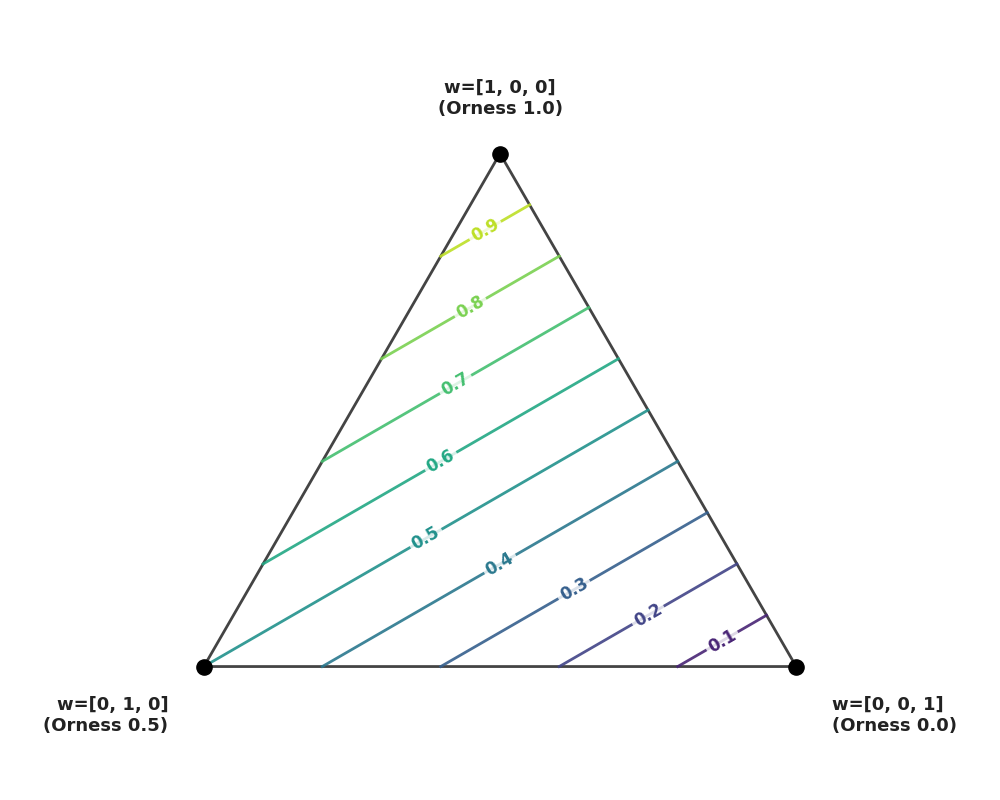
\includegraphics[width=\textwidth]{figures/Orness_in_R3.png}
		\caption{$M=3$: The simplex is a triangle; orness levels correspond to parallel lines.}
	\end{subfigure}
	\hfill
	\begin{subfigure}[b]{0.48\textwidth}
		\centering
		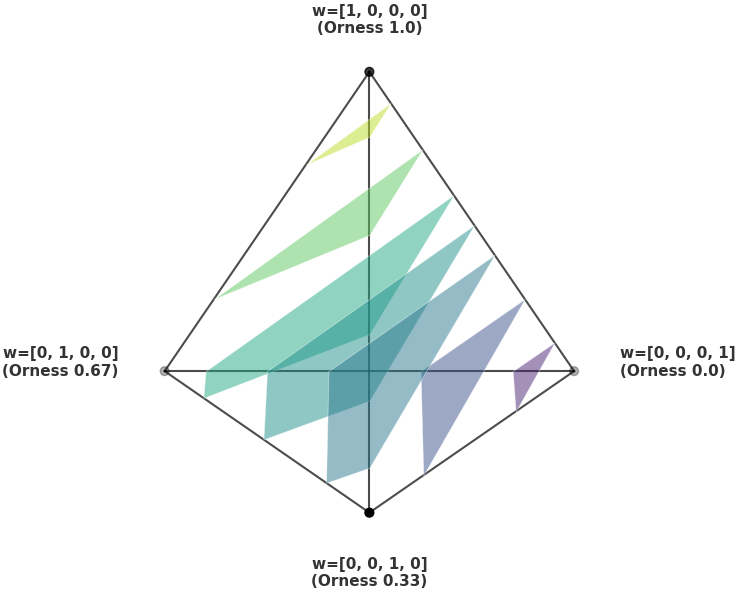
\includegraphics[width=\textwidth]{figures/Orness_in_R4.png}
		\caption{$M=4$: The simplex is a tetrahedron; orness levels correspond to parallel planes.}
	\end{subfigure}
	\caption{Iso-orness hypersurfaces within the weight simplex for $M=3$ and $M=4$ criteria. Each surface contains infinitely many weight vectors sharing the same orness value, illustrating why orness alone cannot uniquely identify a weighting vector.}
	\label{fig:orness_simplex}
\end{figure}


\subsubsection{The Weighted OWA (WOWA) Operator}
%!Igual me pieso si añadir Figuerola-Wischke et al. (2024) donde podríamos decir que WOWA tiene 472 citaciones y 5000 el OWA para decir que tiene mucha más literatura de elicitación o algo así.
Numerous extensions of the OWA operator have been proposed \cite{SurveyEmrouznejad2014}. Many of them rely on viewing the operator from a certain angle \cite{OWAFramework}: as a Choquet integral with respect to symmetric capacities, as a symmetric comonotone additive aggregation function or as a weighted arithmetic mean of ordered inputs. Then, relaxing one or multiple properties lead to a more general and expressive operator, which usually comes at the cost of increased complexity and more parameters to be set. Some frequently used examples include: Generalized OWA \cite{GOWA} replaces the arithmetic mean with the family of power means; Induced OWA \cite{IOWA} performs the ordering based on auxiliary order-inducing variables rather than on the values being aggregated; Fuzzy OWA \cite{FOWA} applies it to fuzzy numbers with level-set arithmetic; and combinations such as the Fuzzy Generalized OWA \cite{FGOWA}.

In particular, in our maintenance scheduling problem, criteria have semantic identity and operational priority, such as grid safety, stability and socio-environmental constraints. Therefore, it is preferred an aggregation model that can explicitly take this structure into account, in addition to the decision-maker's attitudinal behavior. This motivates the use of the Weighted OWA (WOWA) operator, introduced by \citet{WOWA}, which generalizes both the OWA and the weighted arithmetic mean (WAM) by jointly modeling criterion-specific importance and rank-dependent attitudinal behavior.

\begin{definition}[WOWA Operator]
Let $\mathbf{p}=(p_1,\dots,p_M)\in\Delta^{M-1}$ be a criteria importance vector, and let $Q:[0,1]\to[0,1]$ be a linguistic quantifier. Let $\sigma:\{1,\dots,M\}\to\{1,\dots,M\}$ be a permutation such that $x_{(1)}\ge x_{(2)}\ge\cdots\ge x_{(M)}$ and $x_{(j)}=x_{\sigma(j)}$. Define the cumulative importance of $\mathbf{x}$ by $s_0(\mathbf{x})=0$ and $s_j(\mathbf{x})=\sum_{\ell=1}^{j}p_{\sigma(\ell)}$ for $j=1,\dots,M$. The induced WOWA weights are:
\begin{equation}
\label{eq:wowa_weights}
			\omega_j(\mathbf{x})=Q\!\left(s_j(\mathbf{x})\right)-Q\!\left(s_{j-1}(\mathbf{x})\right),\qquad j=1,\dots,M.
\end{equation}
		The operator $\operatorname{WOWA}_{Q,\mathbf{p}}: [0,1]^M \to [0,1]$ is then
		\[
			\operatorname{WOWA}_{Q,\mathbf{p}}(\mathbf{x})=\sum_{j=1}^{M}\omega_j(\mathbf{x})\,x_{(j)}.
		\]
\end{definition}

Notice that the definition of WOWA in the original paper uses 2 weight vectors and an interpolation function, but as stated by the same author in \cite{DirectednessWOWA}, both definitions are equivalent.

The key distinction lies in weight derivation (see Figure~\ref{fig:owa_wowa_weights}). In standard OWA, the quantifier domain $[0,1]$ is partitioned into $M$ intervals of equal width $1/M$. In WOWA, each criterion occupies an interval of width $p_j$: a higher importance yields a wider interval, which captures more of the curvature of $Q$ and thus a larger weight. This mechanism allows the decision-maker to express both an attitudinal profile (via $Q$) and a priority structure (via $p$) simultaneously. Setting $Q(x)\coloneqq x$ recovers the WAM and when $p_j=1/M\,\,\forall j \in \{1,\dots,M\}$, it becomes the OWA.


\begin{figure}[h]
	\centering
	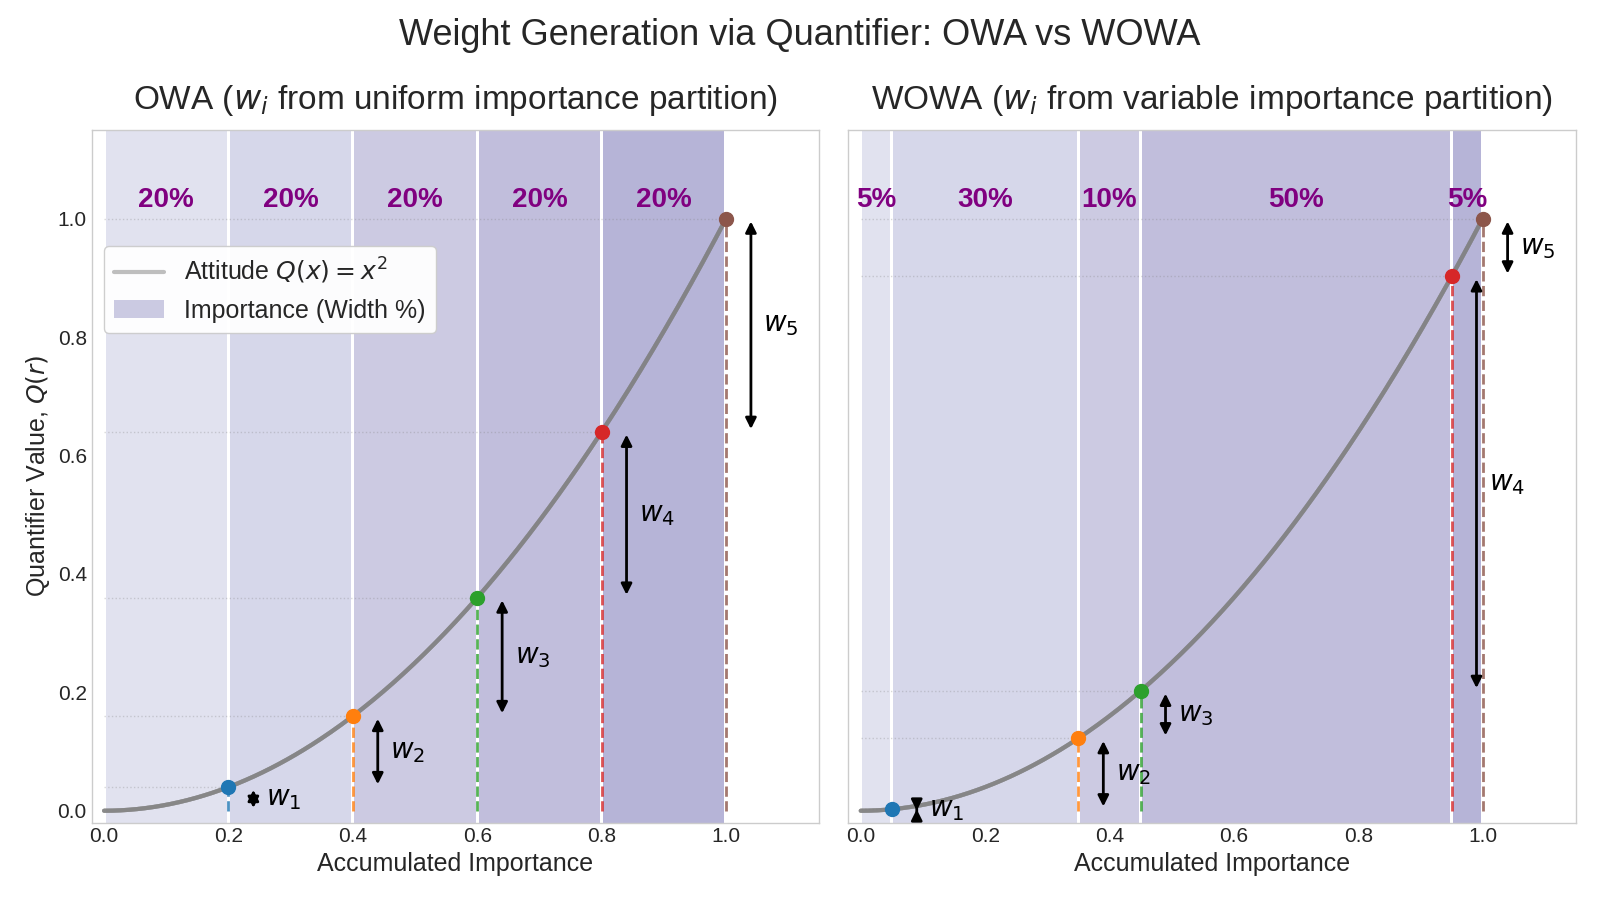
\includegraphics[width=\textwidth]{figures/Weight_Generation_OWA_WOWA.png}
	\caption{Comparison of weight derivation in OWA and WOWA for $M=5$ criteria with $Q(x)=x^2$ (pessimistic attitude). \textbf{Left:} Standard OWA partitions the domain uniformly ($20\%$ each). \textbf{Right:} WOWA uses variable partitions based on criterion importance (e.g., $5\%, 30\%, 10\%, 50\%, 5\%$). The weight $w_j$ corresponds to the vertical increment (black arrows).}
	\label{fig:owa_wowa_weights}
\end{figure}

While learning parameters from reference data for the OWA and WAM operators can be formulated as a quadratic optimization problem (minimization of a squared error distance over a set of examples), this analytical convenience is lost in WOWA \cite{NettletonTorra2001}. The objective function becomes non-quadratic because it relies on an interpolation function that is applied dynamically to the cumulative sums of the importance weights ($\mathbf{p}$) based on the specific ranking permutation ($\sigma$) of the inputs. Accordingly, the Active Set Method formulation cannot be applied, and the authors explicitly remark that, unlike the WAM and OWA cases, it was not known whether the corresponding WOWA distance is convex.

To tackle this complexity, the literature has explored various elicitation approaches. For data-driven learning, \citet{NettletonTorra2001} utilized Genetic Algorithms to approximate the parameters that minimize the prediction error, while \citet{CardinGiove2015} described WOWA weight elicitation as NP-hard in the number of criteria and proposed a Grid-Based Stochastic search to optimize the importance vector alongside a parameterized Monotone Quantifier. 

A different line of work studies scenarios without historical data, where the quantifier can be selected from a desired attitudinal index rather than fitted from examples. \citet{Liu2006} proposes exponential and piecewise-linear quantifier families for WOWA in which the family parameter is uniquely determined by the prescribed orness level. \citet{DirectednessWOWA} studies andness-directed selection across several fuzzy-quantifier families, numerically calibrating each family to a common andness level and showing that different families yield similar outputs in benchmark cases.

These approaches are necessary when operating in the general case, where $Q$ must be treated as a function capable of handling any arbitrary input. However, in Multi-Criteria Decision Making (MCDM) problems involving a specific finite decision matrix, we can adopt a different perspective. The following example illustrates a key insight: for a finite set of alternatives, the WOWA aggregation only requires evaluating \(Q\) at a discrete, finite set of cumulative importance points.

\begin{example}
Consider two alternatives $\mathbf{x}_1=(0.4,0.7,0.5)$ and $\mathbf{x}_2=(0.3,0.9,0.2)$, with criteria importance vector $\mathbf{p}=(0.5,0.2,0.3)$ and quantifier $Q(r)=r^2$.

Sorting $\mathbf{x}_1$ and $\mathbf{x}_2$ yields the ordered vectors $\mathbf{y}_1=(0.7,0.5,0.4)$ and $\mathbf{y}_2=(0.9,0.3,0.2)$. Due to the different sorting permutations, their cumulative importances differ:
\[
s(\mathbf{x}_1) = (0,\, 0.2,\, 0.5,\, 1), \qquad s(\mathbf{x}_2) = (0,\, 0.2,\, 0.7,\, 1).
\]
Consequently, evaluating the increments via equation~\ref{eq:wowa_weights} yields a distinct WOWA weight vector for each alternative: $\omega_1 = (0.04, 0.21, 0.75)$ and $\omega_2 = (0.04, 0.45, 0.51)$, yielding aggregated values:
\begin{alignat*}{2}
\operatorname{WOWA}_{Q,\mathbf{p}}(\mathbf{x}_1) & = \omega_1 \cdot \mathbf{y}_1
		&\quad & = 0.04 \cdot 0.7 + 0.21 \cdot 0.5 + 0.75 \cdot 0.4 \\
		&
		&\quad & = 0.04 \cdot 0.7 + 0.21 \cdot 0.5 + (0.24 + 0.51) \cdot 0.4 = 0.433 \\[0.5em]
\operatorname{WOWA}_{Q,\mathbf{p}}(\mathbf{x}_2) & = \omega_2 \cdot \mathbf{y}_2
		&\quad & = 0.04 \cdot 0.9 + 0.45 \cdot 0.3 + 0.51 \cdot 0.2 \\
		&
		&\quad & = 0.04 \cdot 0.9 + (0.21 + 0.24) \cdot 0.3 + 0.51 \cdot 0.2 = 0.273
\end{alignat*}

As illustrated above, the distributive property allows us to express both aggregations using a common weight vector. This shared vector is derived by evaluating the increments of $Q$ over the union of their cumulative importance points, $\Omega = \bigcup_{i=1}^{2}\{s_j(\mathbf{x}_i):j=0,\dots,3\} = \{0,\, 0.2,\, 0.5,\, 0.7,\, 1\}$, which yields:
\[
\mathbf{W} = \bigl(Q(0.2)-Q(0), \dots, Q(1)-Q(0.7)\bigr) = (0.04,\, 0.21,\, 0.24,\, 0.51)
\]

To align the alternatives with this unified weight space, we simply repeat the values of the sorted vectors $\mathbf{y}_i$ wherever an interval from $s(\mathbf{x}_i)$ is split by $\Omega$:
\[
\mathbf{z}_1 = (0.7,\, 0.5,\, 0.4,\, 0.4), \qquad \mathbf{z}_2 = (0.9,\, 0.3,\, 0.3,\, 0.2).
\]
Now, both alternatives can be computed elegantly as standard dot products using the same weight vector $\mathbf{W}$:
\begin{align*}
\operatorname{WOWA}_{Q,\mathbf{p}}(\mathbf{x}_1) &= \mathbf{W} \cdot \mathbf{z}_1 = 0.04 \cdot 0.7 + 0.21 \cdot 0.5 + 0.24 \cdot 0.4 + 0.51 \cdot 0.4 = 0.433 \\
\operatorname{WOWA}_{Q,\mathbf{p}}(\mathbf{x}_2) &= \mathbf{W} \cdot \mathbf{z}_2 = 0.04 \cdot 0.9 + 0.21 \cdot 0.3 + 0.24 \cdot 0.3 + 0.51 \cdot 0.2 = 0.273
\end{align*}
Essentially, the $\operatorname{WOWA}_{Q,\mathbf{p}}$ aggregation over the original inputs $\{\mathbf{x}_1, \mathbf{x}_2\}$ is equivalent to $\operatorname{OWA}_{\mathbf{W}}$ over the augmented vectors $\{\mathbf{z}_1, \mathbf{z}_2\}$. In this higher-dimensional space, the weights $\mathbf{W}$ correspond to segments of cumulative importance $\Omega$ defined by permutations of $\mathbf{p}$. If a specific criterion's importance spans multiple segments, its value is simply repeated in $\mathbf{z}_i$.
\end{example}
Consequently, for the fixed finite set of alternatives under analysis, the relevant information from $Q$ is fully captured by the increment vector $\mathbf{W}$ on the unified grid $\Omega$. The practical implications go beyond computational convenience. By expressing all alternatives in a unified weight-space representation, the transformation restores the geometric structure needed for the stability analysis developed in section~\ref{sec:selection}.



\subsection{An Exact Unified Weight-Space Representation of WOWA for Finite Choice Sets}
\label{sec:wowa_theorem}

Building on the intuition from the previous example, the transformation is now formalized in theorem \ref{thm:wowa} for an arbitrary fixed decision matrix. Given a set of alternatives $A = \{a_1, \dots, a_N\}$ and a criteria importance vector $\mathbf{p} = (p_1, \dots, p_M)\in \Delta^{M-1}$, it follows:


\begin{definition}[Unified Importance Grid]
	\label{def:grid}
		The unified importance grid $\Omega$ is defined as the union of all breakpoints induced by $\mathbf{p}$ and the sorting $\sigma_i$ of alternatives:
		\[
			\Omega=\bigcup_{i=1}^{N}\{s_j(\mathbf{x}_i):j=0,\dots,M\}=\{0=t_0<\dots<t_K=1\}
		\]
		where $s_0(\mathbf{x}_i)=0$ and $s_j(\mathbf{x}_i)=\sum_{\ell=1}^{j} p_{\sigma_i(\ell)}$ is the cumulative importance of alternative $a_i$ up to the $j$-th sorted criterion, and $K = |\Omega| - 1$ is the number of intervals in the grid.
\end{definition}

\begin{theorem}
	\label{thm:wowa}
		Consider the $\operatorname{WOWA}_{Q,\mathbf{p}}$ operator acting on $\{\mathbf{x}_1,\dots,\mathbf{x}_N\}$. Let $\Omega = \{t_k\}_{k=0}^K$ be the unified importance grid from Definition \ref{def:grid}.

		There exists a $K$-dimensional $\operatorname{OWA}_\mathbf{W}$ operator acting on $\{\mathbf{z}_1,\dots,\mathbf{z}_N\}$ where $z_{ik} = x_{i(j)}$ with $j$ the unique index such that $[t_{k-1}, t_k] \subseteq [s_{j-1}(\mathbf{x}_i), s_j(\mathbf{x}_i)]$ and the weighting vector $\mathbf{W}\in\Delta^{K-1}$ is given by
		\[
			W_k = Q(t_k) - Q(t_{k-1}) \quad \text{for } k \in \{1, \dots, K\}
		\]
		%The existence and uniqueness of such $j$ is guaranteed by the construction of the grid $\Omega$, which implies that each grid interval is entirely contained within exactly one cumulative-importance interval of $\mathbf{x}_i$.

		Then the WOWA operator is equivalent to the higher-dimensional OWA:
		\[
			\operatorname{WOWA}_{Q,\mathbf{p}}(\mathbf{x}_i)=\operatorname{OWA}_{\mathbf{W}}(\mathbf{z}_i)=\sum_{k=1}^K W_k z_{ik},\quad \forall i\in\{1,\dots,N\}
		\]
\end{theorem}

\begin{proof}
		By definition, the WOWA aggregation is:
		\[ \operatorname{WOWA}_{Q,\mathbf{p}}(\mathbf{x}_i)=\sum_{j=1}^M x_{i(j)}\left(Q(s_j(\mathbf{x}_i))-Q(s_{j-1}(\mathbf{x}_i))\right) \]
		Since every cumulative priority $s_j(\mathbf{x}_i)$ belongs to the grid $\Omega = \{t_0, t_1, \ldots, t_K\}$ by construction, there exist indices $\ell_0 < \ell_1 < \cdots < \ell_M$ such that $s_j(\mathbf{x}_i) = t_{\ell_j}$ for each $j \in \{0, \ldots, M\}$, with $\ell_0 = 0$ and $\ell_M = K$.

		For each criterion $j$, define $S_j = \{\ell_{j-1}+1, \ldots, \ell_j\}$ as the set of grid indices whose intervals partition $[s_{j-1}(\mathbf{x}_i), s_j(\mathbf{x}_i)]$. Since these grid intervals are contiguous and cover exactly $[s_{j-1}(\mathbf{x}_i), s_j(\mathbf{x}_i)]$, the WOWA weight decomposes as:
		\[ Q(s_j(\mathbf{x}_i)) - Q(s_{j-1}(\mathbf{x}_i)) = \sum_{k \in S_j} \left( Q(t_k) - Q(t_{k-1}) \right) = \sum_{k \in S_j} W_k \]
		Substituting into the WOWA expression:
		\[ \operatorname{WOWA}_{Q,\mathbf{p}}(\mathbf{x}_i)=\sum_{j=1}^M x_{i(j)}\sum_{k \in S_j} W_k \]

		The sets $S_1, \ldots, S_M$ form a partition of $\{1, \ldots, K\}$, so each grid index $k$ belongs to exactly one $S_j$. This defines a surjective mapping $k \mapsto j$, where $j$ is the unique index satisfying $k \in S_{j}$, or equivalently, $[t_{k-1}, t_k] \subseteq [s_{j-1}(\mathbf{x}_i), s_{j}(\mathbf{x}_i)]$. The double sum can therefore be rewritten by iterating over the finer partition:
		\[ \operatorname{WOWA}_{Q,\mathbf{p}}(\mathbf{x}_i)=\sum_{k=1}^K W_k\cdot x_{i(j)} \]

		By definition of $z_{ik}$ and $j$, it follows that $z_{ik} = x_{i(j)}$.
		Substituting this identity concludes the proof:
		\[ \operatorname{WOWA}_{Q,\mathbf{p}}(\mathbf{x}_i)=\sum_{k=1}^K W_k z_{ik}=\operatorname{OWA}_{\mathbf{W}}(\mathbf{z}_i) \]
	\end{proof}

Notice that the dimension $K$ of the transformed problem is determined by the grid size $|\Omega|-1$. Assuming all criteria have non-zero importance, the dimension satisfies $M \le K \le N \times M$. This dimensionality increase can make the problem intractable for large numbers of criteria and alternatives, where the dynamic computation with multiple weight vectors from the original work is preferred.


The approach established in Theorem~\ref{thm:wowa} is not limited to the WOWA operator, it extends to other aggregation functions that rely on quantifiers and importance weights:

\begin{corollary}
	\label{cor:gwowa_powa}
	Theorem~\ref{thm:wowa} holds for the Generalized WOWA (GWOWA) \cite{GWOWA} and the Prioritized OWA (POWA) \cite{POWA} operators. 
\end{corollary}

\begin{proof}
		For GWOWA, which replaces the arithmetic mean with power means, the aggregation $\left( \sum_j w_j x_{i(j)}^\lambda \right)^{1/\lambda}$ maintains the distributive property over the exponentiated inputs, allowing the exact same weight decomposition. For POWA, where the importance vector $\mathbf{p}_i$ is alternative-dependent (computed based on the satisfaction of higher-priority criteria), once $\Omega$ is constructed, the identical procedure applies.
	\end{proof}
